% -*- latex -*-

\chapter{Build and Install \VTKm}
\label{chap:BuildAndInstall}

Before we begin describing how to develop with \VTKm, we have a brief overview of how to build \VTKm, optionally install it on your system, and start your own programs that use \VTKm.


\section{Getting \VTKm}

\VTKm is an open source software product where the code is made freely available.
To get the latest released version of \VTKm, go to the \VTKm releases page:

\begin{quote}
  \url{http://m.vtk.org/index.php/VTK-m_Releases}
\end{quote}

For access to the most recent work, the \VTKm development team provides public anonymous read access to their main source code repository.
The main \VTKm repository on a gitlab instance hosted at Kitware, Inc.
The repository can be browsed from its project web page:

\begin{quote}
  \url{https://gitlab.kitware.com/vtk/vtk-m}
\end{quote}

\index{git|(}

The source code in the \VTKm repository is access through the \textfilename{git} version control tool.
If you have not used \textfilename{git} before, there are several resources available to help you get familiar with it.
Github has a nice setup guide (\url{https://help.github.com/articles/set-up-git}) to help you get up and running quickly.
For more complete documentation, we recommend the \emph{Pro Git} book (\url{https://git-scm.com/book}).

To get a copy of the \VTKm repository, issue a git clone command.

\begin{blankexample}{Cloning the main \VTKm git repository.}
git clone https://gitlab.kitware.com/vtk/vtk-m.git
\end{blankexample}

The git clone command will create a copy of all the source code to your local machine.
As time passes and you want to get an update of changes in the repository, you can do that with the git pull command.

\begin{blankexample}{Updating a git repository with the pull command.}
git pull
\end{blankexample}

\begin{didyouknow}
  The proceeding examples for using git are based on the \textfilename{git} command line tool, which is particularly prevalent on Unix-based and Mac systems.
  There also exist several GUI tools for accessing git repositories.
  These tools each have their own interface and they can be quite different.
  However, they all should have roughly equivalent commands named ``clone'' to download a repository given a url and ``pull'' to update an existing repository.
\end{didyouknow}

\index{git|)}


\section{Configure \VTKm}
\label{sec:ConfigureVTKm}

\index{CMake|(}
\index{CMake!configuration|(}

\VTKm uses a cross-platform configuration tool named CMake to simplify the configuration and building across many supported platforms.
CMake is available from many package distribution systems and can also be downloaded for many platforms from \url{http://cmake.org}.

Most distributions of CMake come with a convenient GUI application (\textfilename{cmake-gui}) that allows you to browse all of the available configuration variables and run the configuration.
Many distributions also come with an alternative terminal-based version (\textfilename{ccmake}), which is helpful when accessing remote systems where creating GUI windows is difficult.

One helpful feature of CMake is that it allows you to establish a build directory separate from the source directory, and the \VTKm project requires that separation.
Thus, when you run CMake for the first time, you want to set the build directory to a new empty directory and the source to the downloaded or cloned files.
The following example shows the steps for the case where the \VTKm source is cloned from the git repository.
(If you extracted files from an archive downloaded from the \VTKm web page, the instructions are the same from the second line down.)

\begin{blankexample}[ex:RunningCMake]{Running CMake on a cloned \VTKm repository.}
git clone https://gitlab.kitware.com/vtk/vtk-m.git
mkdir vtkm-build
cd vtkm-build
cmake-gui ../vtk-m
\end{blankexample}

\begin{figure}[htb]
  \centering
  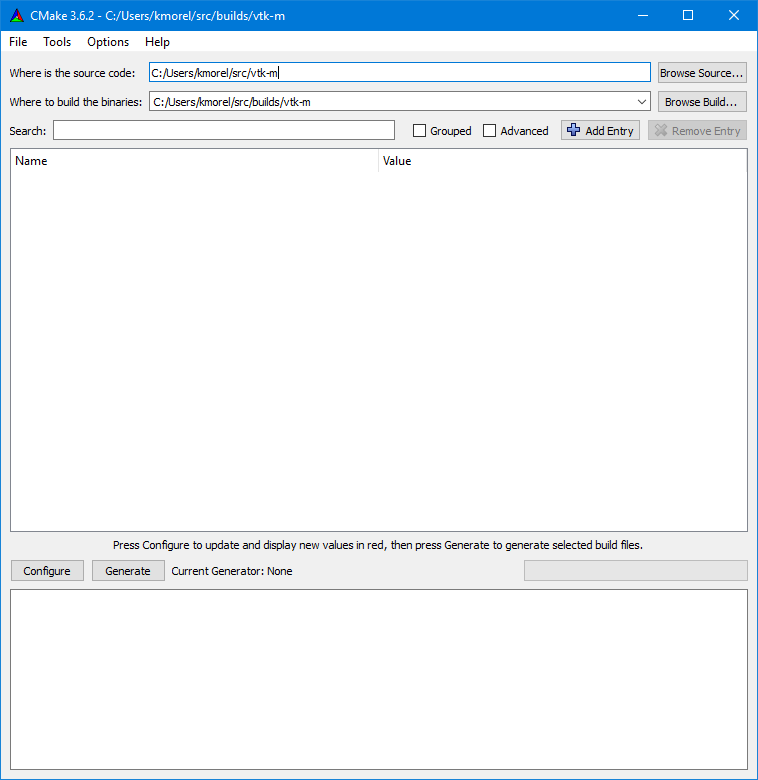
\includegraphics[width=.49\linewidth]{images/CMakeGUIBlank}
  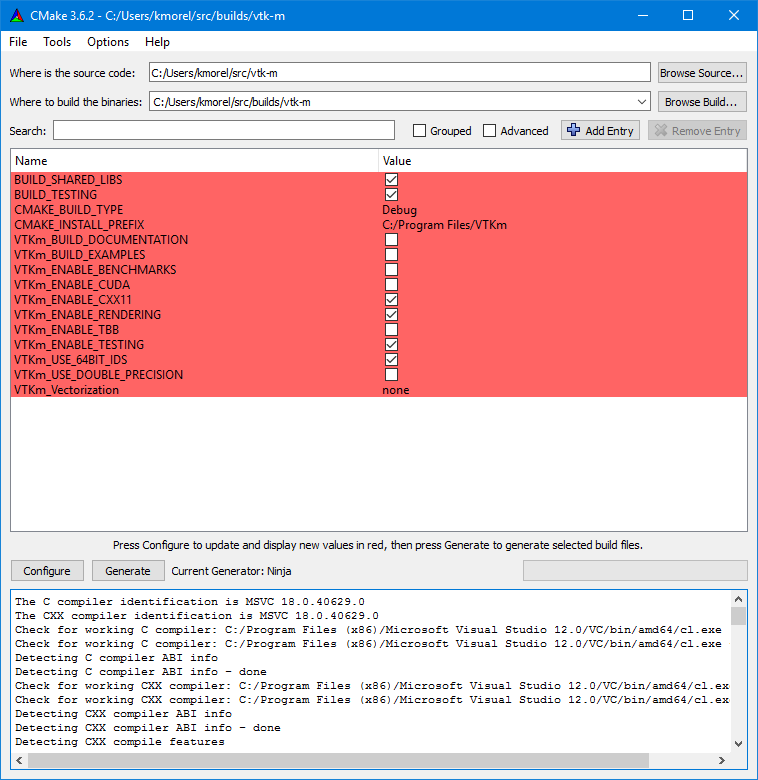
\includegraphics[width=.49\linewidth]{images/CMakeGUI}
  \caption[The CMake GUI configuring the \VTKm project.]{
    The CMake GUI configuring the \VTKm project.
    At left is the initial blank configuration.
    At right is the state after a configure pass.
  }
  \label{fig:CMakeGUI}
\end{figure}

The first time the CMake GUI runs, it initially comes up blank as shown at left in Figure~\ref{fig:CMakeGUI}.
Verify that the source and build directories are correct (located at the top of the GUI) and then click the ``Configure'' button near the bottom.
The first time you run configure, CMake brings up a dialog box asking what generator you want for the project.
This allows you to select what build system or IDE to use (e.g. make, ninja, Visual Studio).
Once you click ``Finish,'' CMake will perform its first configuration.
Don't worry if CMake gives an error about an error in this first configuration process.

\begin{commonerrors}
  Most options in CMake can be reconfigured at any time, but not the compiler and build system used.
  These must be set the first time configure is run and cannot be subsequently changed.
  If you want to change the compiler or the project file types, you will need to delete everything in the build directory and start over.
\end{commonerrors}

After the first configuration, the CMake GUI will provide several configuration options as shown in Figure~\ref{fig:CMakeGUI} on the right.
You now have a chance to modify the configuration of \VTKm, which allows you to modify both the behavior of the compiled \VTKm code as well as find components on your system.
Using the CMake GUI is usually an iterative process where you set configuration options and re-run ``Configure.''
Each time you configure, CMake might find new options, which are shown in red in the GUI.

It is often the case during this iterative configuration process that configuration errors occur.
This can occur after a new option is enabled but CMake does not automatically find the necessary libraries to make that feature possible.
For example, to enable TBB support, you may have to first enable building TBB, configure for TBB support, and then tell CMake where the TBB include directories and libraries are.

Once you have set all desired configuration variables and resolved any CMake errors, click the ``Generate'' button. This will create the build files (such as makefiles or project files depending on the generator chosen at the beginning). You can then close the CMake GUI.

There are a great number of configuration parameters available when running CMake on \VTKm.
The following list contains the most common configuration parameters.

\begin{description}
\item[\cmakevar{BUILD\_SHARED\_LIBS}]
  Determines whether static or shared libraries are built.
\item[\cmakevar{CMAKE\_BUILD\_TYPE}]
  \index{Debug} \index{Release}
  Selects groups of compiler options from categories like Debug and Release.
  Debug builds are, obviously, easier to debug, but they run \emph{much} slower than Release builds.
  Use Release builds whenever releasing production software or doing performance tests.
\item[\cmakevar{CMAKE\_INSTALL\_PREFIX}]
  The root directory to place files when building the install target.
\item[\cmakevar{VTKm\_BUILD\_EXAMPLES}]
  The \VTKm repository comes with an \textfilename{examples} directory.
  This macro determines whether they are built.
\item[\cmakevar{VTKm\_ENABLE\_BENCHMARKS}]
  If on, the \VTKm build includes several benchmark programs.
  The benchmarks are regression tests for performance.
\item[\cmakevar{VTKm\_ENABLE\_CUDA}]
  \index{CUDA}
  Determines whether \VTKm is built to run on CUDA GPU devices.
\item[\cmakevar{VTKm\_ENABLE\_RENDERING}]
  Determines whether to build the rendering library.
\item[\cmakevar{VTKm\_ENABLE\_TBB}]
  Determines whether \VTKm is built to run on multi-core x86 devices using the Intel Threading Building Blocks library.
\item[\cmakevar{VTKm\_ENABLE\_TESTING}]
  If on, the \VTKm build includes building many test programs.
  The \VTKm source includes hundreds of regression tests to ensure quality during development.
\item[\cmakevar{VTKm\_USE\_64BIT\_IDS}]
  If on, then \VTKm will be compiled to use 64-bit integers to index arrays and other lists.
  If off, then \VTKm will use 32-bit integers.
  32-bit integers take less memory but could cause failures on larger data.
\item[\cmakevar{VTKm\_USE\_DOUBLE\_PRECISION}]
  If on, then \VTKm will use double precision (64-bit) floating point numbers for calculations where the precision type is not otherwise specified.
  If off, then single precision (32-bit) floating point numbers are used.
  Regardless of this setting, \VTKm's templates will accept either type.
\end{description}

\index{CMake!configuration|)}
\index{CMake|)}


\section{Building \VTKm}

Once CMake successfully configures \VTKm and generates the files for the build system, you are ready to build \VTKm.
As stated earlier, CMake supports generating configuration files for several different types of build tools.
Make and ninja are common build tools, but CMake also supports building project files for several different types of integrated development environments such as Microsoft Visual Studio and Apple XCode.

The \VTKm libraries and test files are compiled when the default build is invoked.
For example, if \textfilename{Makefile}s were generated, the build is invoked by calling \textfilename{make} in the build directory.
Expanding on Example~\ref{ex:RunningCMake}

\begin{blankexample}[ex:RunningMake]{Using \textfilename{make} to build \VTKm.}
git clone https://gitlab.kitware.com/vtk/vtk-m.git
mkdir vtkm-build
cd vtkm-build
cmake-gui ../vtk-m
make -j
make test
make install
\end{blankexample}

\begin{didyouknow}
  The \textfilename{Makefile}s and other project files generated by CMake support parallel builds, which run multiple compile steps simultaneously.
  On computers that have multiple processing cores (as do almost all modern computers), this can significantly speed up the overall compile.
  Some build systems require a special flag to engage parallel compiles.
  For example, \textfilename{make} requires the \textfilename{-j} flag to start parallel builds as demonstrated in Example~\ref{ex:RunningMake}.
\end{didyouknow}

\begin{commonerrors}
  CMake allows you to switch between several types of builds including default, Debug, and Release.
  Programs and libraries compiled as release builds can run \emph{much} faster than those from other types of builds.
  Thus, it is important to perform Release builds of all software released for production or where runtime is a concern.
  Some integrated development environments such as Microsoft Visual Studio allow you to specify the different build types within the build system.
  But for other build programs, like \textfilename{make}, you have to specify the build type in the \cmakevar{CMAKE\_BUILD\_TYPE} CMake configuration variable, which is described in Section~\ref{sec:ConfigureVTKm}.
\end{commonerrors}

CMake creates several build ``targets'' that specify the group of things to build.
The default target builds all of \VTKm's libraries as well as tests, examples, and benchmarks if enabled.
The \textfilename{test} target executes each of the \VTKm regression tests and verifies they complete successfully on the system.
The \textfilename{install} target copies the subset of files required to use \VTKm to a common installation directory.
The \textfilename{install} target may need to be run as an administrator user if the installation directory is a system directory.

\begin{didyouknow}
  A good portion of \VTKm is a header-only library, which does not need to be built in a traditional sense.
  However, \VTKm contains a significant amount of tests to ensure that the header code does compile and run correctly on a given system.
  If you are not concerned with testing a build on a given system, you can turn off building the testing, benchmarks, and examples using the CMake configuration variables described in Section~\ref{sec:ConfigureVTKm}.
  This can shorten the \VTKm compile time.
\end{didyouknow}


\section{Linking to \VTKm}

Ultimately, the value of \VTKm is the ability to link it into external projects that you write.
The header files and libraries installed with \VTKm are typical, and thus you can link \VTKm into a software project using any type of build system.
However, \VTKm comes with several CMake configuration files that simplify linking \VTKm into another project that is also managed by CMake.
Thus, the documentation in this section is specifically for finding and configuring \VTKm for CMake projects.

\index{CMake|(}
\index{CMake!VTK-m package|(}
\index{VTK-m CMake package|(}

\VTKm can be configured from an external project using the \textcode{find\_package} CMake function.
The behavior and use of this function is well described in the CMake documentation.
The first argument to \textcode{find\_package} is the name of the package, which in this case is \textcode{VTKm}.
CMake configures this package by looking for a file named \textfilename{VTKmConfig.cmake}, which will be located in the \textfilename{lib} directory of the install or build of \VTKm.
The configurable CMake variable \cmakevar{VTKm\_DIR} can be set to the directory that contains this file.

\begin{didyouknow}
  The CMake \textcode{find\_package} function also supports several features not discussed here including specifying a minimum or exact version of \VTKm and turning off some of the status messages.
  See the CMake documentation for more details.
\end{didyouknow}

\index{CMake!VTK-m package!components|(}
\index{VTK-m CMake package!components|(}

\newcommand*{\cmakecomponent}[1]{%
  \textsf{#1}%
  \index{#1}%
  \index{CMake!VTK-m package!#1}%
  \index{VTK-m CMake package!components!#1}}

The CMake package for VTK-m is broken down into components that let you load particular features of VTK-m.
Package components can be specified with the \textcode{COMPONENTS} and \textcode{OPTIONAL\_COMPONENTS} arguments to the \textcode{find\_package} function.
The following example demonstrates using \textcode{find\_package} to find the \VTKm package that requires the \cmakecomponent{Serial} backend as well as the \cmakecomponent{Rendering} and \cmakecomponent{OpenGL} features as well as optionally using the \cmakecomponent{TBB} and \cmakecomponent{CUDA} backends.

\begin{blankexample}{Loading \VTKm configuration from an external CMake project.}
find_package(VTKm REQUIRED
  COMPONENTS Serial OpenGL Rendering
  OPTIONAL_COMPONENTS TBB CUDA
  )
\end{blankexample}

The following components are available.
Many of the features for these components are described elsewhere within this book.

\begin{description}
\item[\cmakecomponent{Base}]
  The ``base'' configuration required for using any part of \VTKm.
  This component is loaded automatically even if no components are specified in \textcode{find\_package}.
\item[\cmakecomponent{Serial}]
  The serial backend for \VTKm, which is useful for debugging and when no other backend is available.
\item[\cmakecomponent{OpenGL}]
  Support for the integration of OpenGL features with \VTKm.
\item[\cmakecomponent{OSMesa}]
  Support for creating off screen canvases using the OSMesa library.
\item[\cmakecomponent{EGL}]
  Support for creating off screen canvases using the EGL library.
\item[\cmakecomponent{GLFW}]
  A convenience component that loads the necessary configuration to use the GLFW library, which provides a cross-platform interface for creating OpenGL windows.
\item[\cmakecomponent{GLUT}]
  A convenience component that loads the necessary configuration to use the GLUT library, which provides a cross-platform interface for creating OpenGL windows.
\item[\cmakecomponent{Interop}]
  Support for transferring \VTKm array data directly to OpenGL objects.
\item[\cmakecomponent{Rendering}]
  Use of the lightweight \VTKm rendering library, which provides basic rendering of \VTKm data objects.
\item[\cmakecomponent{TBB}]
  The Intel Threading Building Blocks (TBB) backend for \VTKm, which uses multiple cores and threads for parallel processing.
\item[\cmakecomponent{CUDA}]
  The CUDA backend for \VTKm, which uses GPU processors for parallel processing.
\end{description}

\index{VTK-m CMake package!components|)}
\index{CMake!VTK-m package!components|)}

\newcommand*{\cmakevtkmpackagevariable}[1]{%
  \textsf{#1}%
  \index{#1}%
  \index{CMake!VTK-m package!#1}%
  \index{VTK-m CMake package!variables!#1}}

After the \textcode{find\_package} function completes, C++ libraries and executables can be creating using the configuration variables defined.
The following is a simple example of creating an executable.

\begin{blankexample}{Loading \VTKm configuration from an external CMake project.}
find_package(VTKm REQUIRED
  COMPONENTS Serial OpenGL Rendering
  OPTIONAL_COMPONENTS TBB CUDA
  )

add_executable(myprog myprog.cxx)
target_include_directories(myprog PRIVATE ${VTKm_INCLUDE_DIRS})
target_link_libraries(myprog ${VTKm_LIBRARIES})
target_compile_options(myprog PRIVATE ${VTKm_COMPILE_OPTIONS})
\end{blankexample}

\begin{commonerrors}
  It is not sufficient to just call \textcode{find\_package} to compile code using \VTKm.
  You must also use the \cmakevtkmpackagevariable{VTKm\_INCLUDE\_DIRS} and \cmakevtkmpackagevariable{VTKm\_LIBRARIES} CMake variables to configure the compiler to load \VTKm's components.
  (Although technically not required, it is highly advisable to also use the \cmakevtkmpackagevariable{VTKm\_COMPILE\_OPTIONS} variable as well.) 
\end{commonerrors}

\index{CMake!VTK-m package!variables|(}
\index{VTK-m CMake package!variables|(}

The following is a list of all the CMake variables defined when the \textcode{find\_package} function completes.

\begin{description}
\item[\cmakevtkmpackagevariable{VTKm\_FOUND}]
  Set to true if the \VTKm CMake package, all its dependent packages, and all the specified components were successfully configured.
  If \textcode{find\_package} was not called with the \textcode{REQUIRED} option, then this variable should be checked before attempting to use \VTKm.
\item[\cmakevtkmpackagevariable{VTKm\_{\it{}\textless{}component\_name\textgreater{}}\_FOUND}]
  For each component specified in the \textcode{find\_package} call, one of these variables will be defined as true or false depending on whether the component successfully loaded.
  For components specified as an \textcode{OPTIONAL\_COMPONENTS} argument, the \cmakevtkmpackagevariable{VTKm\_FOUND} might still be true (because all required components succeeded) while the associated \cmakevtkmpackagevariable{VTKm\_{\it{}\textless{}component\_name\textgreater{}}\_FOUND} could be false if that specific component failed to load.
\item[\cmakevtkmpackagevariable{VTKm\_INCLUDE\_DIRS}]
  Contains a list of all directories that need to be specified to properly include \VTKm header files.
  These also include the directories needed for header files that \VTKm depends on and specified components.
  Targets should use the \textcode{target\_include\_directories} CMake function to add this list of directories to the compile commands.
\item[\cmakevtkmpackagevariable{VTKm\_LIBRARIES}]
  Contains a list of all requested \VTKm libraries and component libraries.
  Targets should use the \textcode{target\_link\_libraries} CMake function to add this list of libraries to the link commands.
\item[\cmakevtkmpackagevariable{VTKm\_COMPILE\_OPTIONS}]
  Contains a string of options that \VTKm suggests to add to the compiler.
  Targets should use the \textcode{target\_compile\_options} CMake function to add this list of options to the compile commands.
\end{description}

\index{VTK-m CMake package!variables|)}
\index{CMake!VTK-m package!variables|)}

\index{VTK-m CMake package|)}
\index{CMake!VTK-m package|)}
\index{CMake|)}
